\documentclass{article}
\usepackage[margin=1in]{geometry}
\usepackage{enumitem}
\usepackage{setspace}
\usepackage{amsmath}
\usepackage{amssymb}
\usepackage{physics}
\usepackage{graphicx}

\title{Math 132 Homework 3}
\date{10/20/2020}
\author{Jiaping Zeng}

\begin{document}
\setstretch{1.35}
\maketitle

\begin{itemize}
      \item [2.4.33] Suppose that $f=u+iv$ is analytic in a region $\Omega$. Show that
            \begin{itemize}
                  \item [(a)] $f'(z)=u_x-iu_y$, also $f'(z)=v_y+iv_x$\\
                        \textbf{Answer}: By Cauchy-Riemann equations, we have $u_x=v_y$ and $u_y=-v_x$. Starting from $f'(z)=u_x+iv_x$ (differentiate $f$ with respect to $x$), we can substitute in $v_x=-iv_y$, which give us $f'(z)=u_x-iu_y$. Similarly, we can substitute in $u_x=v_y$, which gives us $f'(z)=v_y+iv_x$.
                  \item [(b)] $\abs{f'(z)}^2=u_x^2+u_y^2=v_x^2+v_y^2$\\
                        \textbf{Answer}: From part (a), $f'(z)=u_x-iu_y\implies\abs{f'(z)}^2=(\sqrt{u_x^2+u_y^2})^2=u_x^2+u_y^2$; similarly, $f'(z)=v_y+iv_x\implies\abs{f'(z)}^2=(\sqrt{v_x^2+v_y^2})^2=v_x^2+v_y^2$.
                  \item [(c)] Conclude from (a) or (b) that either $\Re f$ or $\Im f$ is constant in $\Omega$, then $f$ is constant in $\Omega$.\\
                        \textbf{Answer}: On the one hand, if $\Re f=u$ is constant, we have $u_x=u_y=0\implies\abs{f'(z)}^2=u_x^2+u_y^2=0$. On the other hand, if $\Im f=v$ is constant, we have $v_x=v_y=0\implies\abs{f'(z)}=v_x^2+v_y^2=0$. Since the magnitude of the $f'(z)$ is $0$ in either case, $f'(z)$ is constant in $\Omega$.
            \end{itemize}
      \item [2.5.3] $e^x\cos y$\\
            \textbf{Answer}: Let $u=e^x\cos x$, then $\Delta u=\frac{\delta^2 u}{\delta x^2}+\frac{\delta^2 u}{\delta y^2}=\frac{\delta}{\delta x}(e^x\cos y)-\frac{\delta}{\delta y}(e^x\sin y)=e^x\cos y-e^x\cos y=0$. Therefore $e^x\cos y$ is harmonic on $\Omega=\mathbb{C}$.
      \item [2.5.14] $x^2-y^2-xy$\\
            \textbf{Answer}: Let $u=x^2-y^2-xy$, then $u_x=2x-y$ and $u_y=-2y-x$. By Cauchy-Riemann, $v$ must satisfy $u_x=v_y\implies v_y=2x-y\implies v=2xy-\frac{1}{2}y^2+c(x)$. Again by Cauchy-Riemann, $v$ must also satisfy $u_y=-v_x\implies -2y-x=-2y-c'(x)\implies c'(x)=x\implies c(x)=\frac{1}{2}x^2+C$. Therefore $v=2xy+\frac{1}{2}x^2-\frac{1}{2}y^2+C$. We can check Cauchy-Riemann as follows:\\
            $u_x=2x-y$, $v_y=2x-y\implies u_x=v_y$\\
            $u_y=-2y-x$, $-v_x=-2y-x\implies u_y=-v_x$
      \item [2.5.19] Show that if $u$ and $u^2$ are both harmonic in a region $\Omega$, then $u$ must be constant.\\
            \textbf{Answer}: Since $u^2$ is harmonic in $\Omega$, we have $\frac{\delta^2}{\delta x^2}(u^2)+\frac{\delta^2}{\delta y^2}(u^2)=0\implies\frac{\delta}{\delta x}(2uu_{x})+\frac{\delta}{\delta y}(2uu_{y})=0\implies 2(uu_{xx}+u_x^2)+2(uu_{yy}+u_y^2)=0\implies u(u_{xx}+u_{yy})+u_x^2+u_y^2=0$. Then, since $u$ is harmonic, we also have $\frac{\delta^2 u}{\delta x^2}+\frac{\delta^2 u}{\delta y^2}=0\implies u_{xx}+u_{yy}=0$. Combining the last two equalities we have $u_x^2+u_y^2=0$, implying that $u_x=u_y=0$ as $u$ is a real function. Therefore $u$ is constant.
      \item [3.1.1] The line segment with initial point $z_1=1+i$ and terminal $z_2=-1-2i$.\\
            \textbf{Answer}: $\gamma(t)=z_0+t(z_1-z_0)=(1+i)-t((1+i)-(-1-2i))=t(-2-3i)+1+i$
            \begin{center}
                  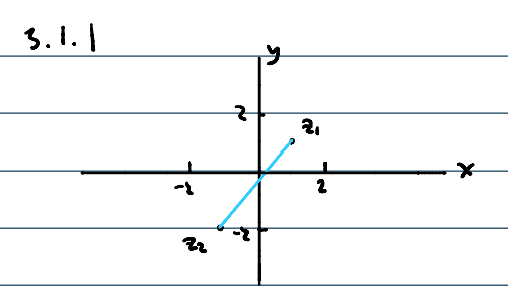
\includegraphics[width=2in]{3-1-1.png}
            \end{center}
      \item [3.1.3] The counterclockwise circle with center at $3i$ and radius $1$.\\
            \textbf{Answer}: $\gamma(t)=z_0+re^{it}=3i+e^{it}$
            \begin{center}
                  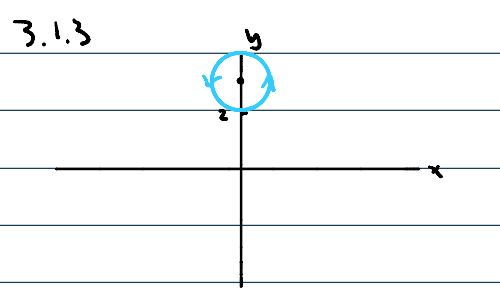
\includegraphics[width=2in]{3-1-3.png}
            \end{center}
      \item [3.1.4] The clockwise circle with center at $-2-i$ and radius $3$.\\
            \textbf{Answer}: $\gamma(t)=z_0+re^{it}=-2-i+3e^{-it}$
            \begin{center}
                  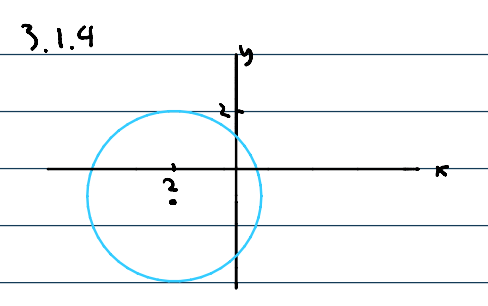
\includegraphics[width=2in]{3-1-4.png}
            \end{center}
      \item [P1] For what values of $z$ is the sequence $\{z^n\}_{n=1}^\infty$ bounded? For which values of $z$ does the sequence converge to $0$?\\
            \textbf{Answer}: Let $r=\abs{z}\in\mathbb{R}$, then as $n\rightarrow\infty$, we have $r\leq 1\implies r^n\leq 1$ and $r>1\implies r^n\rightarrow\infty$. Therefore $\{z^n\}_{n=1}^\infty$ is bounded for $\abs{z}\leq 1$ and unbounded otherwise. Similarly, since $r=\abs{z}\rightarrow 0$ when $r<1$, $\{z^n\}\rightarrow 0$ when $\abs{z}<1$.
      \item [P2] Let $f(z)=\abs{z}^2$ for all $z\in\mathbb{C}$.
            \begin{itemize}
                  \item [(a)] Use the definition of the complex derievative, show that $f$ is not differentiable at any \textbf{nonzero} point $z_0=x_0+iy_0$.\\
                        \textbf{Answer}: $\lim_{h\rightarrow 0}\frac{f(z_0+h)-f(z_0)}{h}=\lim_{h\rightarrow 0}\frac{\abs{z_0+h}^2+\abs{z_0}^2}{h}=\lim_{h\rightarrow 0}\frac{(z_0+h)\overline{(z_0+h)}-z_0\overline{z_0}}{h}$, which evaluates to $0$ only if $z=0$ and has different partial derievatives otherwise.
                  \item [(b)] Use the definition of the complex derievative, show that $f'(0)$ exists.\\
                        \textbf{Answer}: $f'(z_0)=\lim_{h\rightarrow 0}\frac{f(0+h)-f(0)}{h}=\lim_{h\rightarrow 0}\frac{\abs{h}^2}{h}=\lim_{h\rightarrow 0}\frac{h\bar{h}}{h}=\lim_{h\rightarrow 0}\bar{h}=0$.
                  \item [(c)] If $f$ analytic at $z_0=0$?\\
                        \textbf{Answer}: No because $f$ is not differentiable on any open set containing $z_0=0$.
            \end{itemize}
      \item [P3] Show that $f(z)=\bar{z}^2$ does not satisfy the Cauchy-Riemann equations and hence is not analytic on $\mathbb{C}$.\\
            \textbf{Answer}: Let $z=x+iy$, then $f(z)=\bar{z}^2=\overline{x-iy}^2=x^2-y^2-2ixy$. So $u=\Re f=x^2+y^2$ and $v=\Im f=-2xy$. Then we can test the Cauchy-Riemann equations as follows:\\
            $u_x=2x,v_y=-2x\implies u_x\neq -2x$\\
            $u_y=2y,-v_x=2y\implies u_y=-v_x$\\
            Therefore $f(z)=\bar{z}^2$ does not satisfy the Cauchy-Riemann equations and hence is not analytic on $\mathbb{C}$.
      \item [P4] Let $f(z)=z^7-z^5$.
            \begin{itemize}
                  \item [(a)] Recall from lecture the reverse triangle inequality: \[\abs{w-z}\geq\abs{\abs{w}-\abs{z}}\text{ for all }w,z\in\mathbb{C}.\] Use this to show that $\abs{f'(1-i)}\geq 56-20=36$ and hence $f'(1-i)\neq 0$.\\
                        \textbf{Answer}: $f'(z)=7z^6-5z^4\implies\abs{f'(1-i)}=\abs{7(1-i)^6-5(1-i)^4}\geq\abs{7\abs{1-i}^6-5\abs{1-i}^4}=\abs{7\cdot\sqrt{2}^6-5\cdot\sqrt{2}^4}=36\neq 0$.
                  \item [(b)] Combining part (a) with the theorem from class, we see that $f^{-1}$ exists and is analytic near $f(1-i)$. What is $(f^{-1})'((1-i)^7-(1-i)^5)$?\\
                        \textbf{Answer}: Since $f'(1-i)\neq 0$, we have $(f^{-1})'(w)=\frac{1}{f'(f^{-1}(w))}$. Let $w=(1-i)^7-(1-i)^5=z^7-z^5$, then $f^{-1}(w)=z\implies z=1+i$. So $(f^{-1})'(w)=\frac{1}{f'(z)}=\frac{1}{7(1-i)^6-5(1-i)^4}=\frac{1}{-i^7+7i^6-21i^5+35i^4-35i^3+21i^2-7i+1025}$.
            \end{itemize}
      \item [P5] Let $f(z)=e^{z^2}$.
            \begin{itemize}
                  \item [(a)] Find the real and imaginary parts $u$ and $v$ of $f$ so that $f(z)=u(x,y)+iv(x,y)$.\\
                        \textbf{Answer}: Let $z=x+iy$, then $z^2=x^2-y^2+2ixy$. So $f(z)=e^{z^2}=e^{x^2-y^2+2ixy}=e^{x^2-y^2}\cdot e^{2ixy}=e^{x^2-y^2}(\cos(2xy)+i\sin(2xy))=e^{x^2-y^2}\cos(2xy)+ie^{x^2-y^2}\sin(2xy)$. Therefore we have $u=e^{x^2-y^2}\cos(2xy)$ and $v=e^{x^2-y^2}\sin(2xy)$.
                  \item [(b)] Show that $e^{x^2-y^2}\cos(2xy)$ is a harmonic function and find a harmonic conjugate.\\
                        \textbf{Answer}: Let $u=e^{x^2-y^2}\cos(2xy)=e^{x^2}e^{-y^2}\cos(2xy)$, then we need to verify that $\Delta u=\frac{\delta^2 u}{\delta x^2}+\frac{\delta^2 u}{\delta y^2}=0$. Differentiating twice gives us $\frac{\delta^2 u}{\delta x^2}=2e^{x^2-y^2}[(2x^2-2y^2+1)\cos(2xy)-4xy\sin(2xy)]$ and $\frac{\delta^2 u}{\delta y^2}=2e^{x^2-y^2}[4xy\sin(2xy)-(2x^2-2y^2+1)\cos(2xy)]$. Therefore $\frac{\delta^2 u}{\delta x^2}+\frac{\delta^2 u}{\delta y^2}=0$ and $u$ is harmonic.\\
                        We can verify that $v=e^{x^2-y^2}\sin(2xy)$ from part (a) is the harmonic conjugate of $u$ by verifying Cauchy-Riemann:\\
                        $u_x=e^{x^2-y^2}[2x\cos(2xy)-2y\sin(2xy)]=v_y\implies u_x=v_y$\\
                        $u_y=e^{x^2-y^2}[-2x\sin(2xy)-2y\cos(2xy)]=-v_x\implies u_y=-v_x$\\
                        Therefore $v=e^{x^2-y^2}\sin(2xy)$ is the harmonic conjugate of $u$.
            \end{itemize}
      \item [P6] Let $f:D\rightarrow\mathbb{C}$ be an analytic function defined on a region $D$ such that $f'(z)=f(z)$ for all $z\in D$. Show that $f(z)=\alpha e^z$ for some constant $\alpha\in\mathbb{C}$.\\
            \textbf{Answer}: Let $g(z)=e^{-z}f(z)$, then $g'(z)=e^{-z}f'(z)-e^{-z}f(z)$. Since $f'(z)=f(z)$, we have $g'(z)=0$. In addition, since $f$ and $e^{-z}$ are both analytic in $D$, so is $g(z)$. Therefore $g(z)=\alpha$ for some constant $\alpha$ and by substitution we have $e^{-z}f(z)=\alpha\implies f(z)=\alpha e^z$.
      \item [P7] Plot the given path:
            \begin{itemize}
                  \item [(a)] $\gamma(t)=te^{-it}$ for $t\in[0,4\pi]$.\\\textbf{Answer}: Since $e^{-it},t\in[0,4\pi]$ is a doubly traced, clockwise circle, $te^{-it}$ is a clockwise spiral with radius increasing from $0$ to $4\pi$.
                        \begin{center}
                              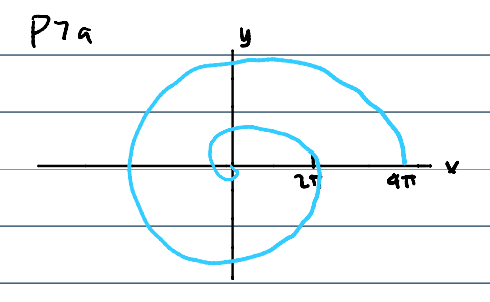
\includegraphics[width=2in]{P7a.png}
                        \end{center}
                  \item [(b)] $\gamma(t)=t+i\sin(\pi t)$ for $t\in[0,2]$.\\\textbf{Answer}: We have $x(t)=t$ and $y(t)=\sin(\pi t)$, so the graph is $y(x)=\sin(x)$ from $0$ to $2\pi$.
                        \begin{center}
                              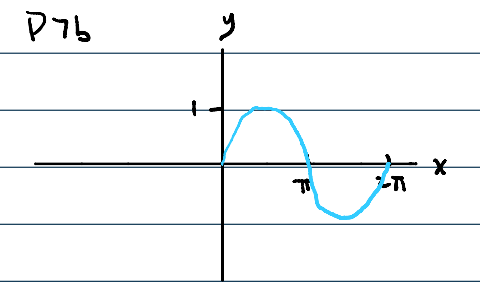
\includegraphics[width=2in]{P7b.png}
                        \end{center}
            \end{itemize}
\end{itemize}
\end{document}